% !TEX program = pdflatex
% =============================================================================
%  Next-Gen Model Risk Management: High-Fidelity Document Intelligence
%  Morgan Stanley — MRM IRD Technology Proposal
%  Author: Alexander Tsoskounoglou
%  Date: February 2026
% =============================================================================
\documentclass[aspectratio=169, 11pt]{beamer}

% ─── Theme & Colors ──────────────────────────────────────────────────────────
\usetheme{Madrid}
\useinnertheme{circles}

% Morgan Stanley brand-approximate palette
\definecolor{MSBlue}{RGB}{0, 43, 92}
\definecolor{MSLightBlue}{RGB}{0, 114, 188}
\definecolor{MSGrey}{RGB}{108, 117, 125}
\definecolor{MSSilver}{RGB}{200, 206, 212}
\definecolor{MSWhite}{RGB}{255, 255, 255}
\definecolor{AccentGreen}{RGB}{46, 184, 92}
\definecolor{AccentRed}{RGB}{220, 53, 69}
\definecolor{AccentAmber}{RGB}{255, 193, 7}
\definecolor{CodeBG}{RGB}{40, 44, 52}

\setbeamercolor{palette primary}{bg=MSBlue, fg=MSWhite}
\setbeamercolor{palette secondary}{bg=MSLightBlue, fg=MSWhite}
\setbeamercolor{palette tertiary}{bg=MSBlue, fg=MSWhite}
\setbeamercolor{palette quaternary}{bg=MSBlue, fg=MSWhite}
\setbeamercolor{structure}{fg=MSBlue}
\setbeamercolor{section in toc}{fg=MSBlue}
\setbeamercolor{title}{fg=MSWhite, bg=MSBlue}
\setbeamercolor{frametitle}{fg=MSWhite, bg=MSBlue}
\setbeamercolor{block title}{bg=MSBlue, fg=MSWhite}
\setbeamercolor{block body}{bg=MSSilver!30, fg=black}
\setbeamercolor{block title alerted}{bg=AccentRed, fg=MSWhite}
\setbeamercolor{block body alerted}{bg=AccentRed!10, fg=black}
\setbeamercolor{block title example}{bg=AccentGreen!70!black, fg=MSWhite}
\setbeamercolor{block body example}{bg=AccentGreen!10, fg=black}
\setbeamercolor{item}{fg=MSLightBlue}
\setbeamercolor{subitem}{fg=MSGrey}

\setbeamertemplate{navigation symbols}{}
\setbeamertemplate{caption}{\raggedright\insertcaption\par} % Fix caption formatting

% Custom footline
\setbeamertemplate{footline}{%
  \leavevmode%
  \hbox{%
    \begin{beamercolorbox}[wd=.333333\paperwidth,ht=2.5ex,dp=1ex,left]{footline}%
      \hspace*{2ex}\scriptsize\textcolor{MSGrey}{Morgan Stanley $|$ Confidential}%
    \end{beamercolorbox}%
    \begin{beamercolorbox}[wd=.333333\paperwidth,ht=2.5ex,dp=1ex,center]{footline}%
      \scriptsize\textcolor{MSGrey}{MRM IRD --- Document Intelligence}%
    \end{beamercolorbox}%
    \begin{beamercolorbox}[wd=.333333\paperwidth,ht=2.5ex,dp=1ex,right]{footline}%
      \scriptsize\textcolor{MSGrey}{\insertframenumber{}/\inserttotalframenumber}\hspace*{2ex}%
    \end{beamercolorbox}%
  }%
  \vskip0pt%
}

% ─── (footer uses \inserttotalframenumber directly) ─────────────────────────

% ─── Packages ────────────────────────────────────────────────────────────────
\usepackage[T1]{fontenc}
\usepackage{lmodern}
\usepackage{amsmath, amssymb, amsfonts}
\usepackage{mathtools}
\usepackage{tikz}
\usetikzlibrary{arrows.meta, positioning, shapes.geometric, calc, fit, backgrounds}
\usepackage{booktabs}
\usepackage{graphicx}
\usepackage{listings}
\usepackage{multicol}
\usepackage{textcomp}

% ─── TikZ Styles ─────────────────────────────────────────────────────────────
\tikzset{
  phase/.style={
    rectangle, rounded corners=6pt, draw=#1, fill=#1!8,
    minimum height=3.0cm, text width=4.0cm, align=left,
    font=\small, line width=1pt, inner sep=5pt
  },
  timeline/.style={thick, color=MSGrey, -{Stealth[length=5pt]}},
}

% ─── Custom icon commands ────────────────────────────────────────────────────
\newcommand{\iconcheck}{\textcolor{AccentGreen!70!black}{$\checkmark$}}
\newcommand{\iconcross}{\textcolor{AccentRed}{$\times$}}
\newcommand{\iconwarn}{\textcolor{AccentAmber}{$\triangle$}}
\newcommand{\iconbullet}{\textcolor{MSLightBlue}{$\blacktriangleright$}}

% ─── Metadata ────────────────────────────────────────────────────────────────
\title[MRM Document Intelligence]{%
  \texorpdfstring{%
    Next-Gen Model Risk Management\\[4pt]
    {\large High-Fidelity Document Intelligence}%
  }{Next-Gen MRM: High-Fidelity Document Intelligence}%
}
\subtitle{Transforming PDF Analysis with AI-Powered Extraction}
\author{Alexander Tsoskounoglou}
\institute[Morgan Stanley]{%
  Associate, Model Risk Management --- Interest Rate Derivatives (MRM IRD)\\
  Morgan Stanley, Budapest
}
\date{February 2026}

% =============================================================================
\begin{document}

% ─── SLIDE 1: Title ─────────────────────────────────────────────────────────
{
\setbeamertemplate{footline}{}
\begin{frame}
\titlepage
\end{frame}
}

% ─── SLIDE 2: Who Am I ──────────────────────────────────────────────────────
\begin{frame}{Who Am I}
\vspace{4pt}
\textbf{\textcolor{MSBlue}{Alexander Tsoskounoglou}}
\vspace{6pt}
\begin{itemize}
  \item \textbf{BSc Computer Science} --- solid foundation in software engineering \& algorithms
  \item \textbf{MSc Computational Finance} (University of Amsterdam) --- quantitative modelling, stochastic calculus \& numerical methods
  \item \textbf{Quantitative Analyst} (1~year, hedge fund) --- developed \& deployed neural-network-based trading strategies in production
  \item \textbf{Quantitative Researcher} (1~year, University of Amsterdam) --- led two research projects on Deep Reinforcement Learning for hedging \& pricing exotic derivatives
\end{itemize}
\end{frame}

% ─── SLIDE 3: The Current Friction ──────────────────────────────────────────
\begin{frame}{The Current Friction: A Wall of PDFs}
\begin{columns}[T]
\begin{column}{0.48\textwidth}
  \begin{block}{The MRM Document Landscape}
    \begin{itemize}
      \item \textbf{Thousands} of model documents in the Model Context System
      \item Bermudian Swaptions, SABR Calibrations, CVA/XVA frameworks\ldots
      \item Dense with:
      \begin{itemize}
        \item[$\bullet$] Multi-line integral equations \& SDEs
        \item[$\bullet$] Stochastic calculus (It\^{o}, martingales)
        \item[$\bullet$] Nested tables of Greeks \& sensitivities
        \item[$\bullet$] \textbf{Figures, charts \& diagrams} --- calibration surfaces, payoff diagrams
      \end{itemize}
    \end{itemize}
  \end{block}
\end{column}
\begin{column}{0.48\textwidth}
  \begin{alertblock}{Why ``Copy-Paste into an LLM'' Fails}
    \begin{enumerate}
      \item \textbf{PDF $\neq$ Text} --- PDFs store glyphs, not semantics
      \item \textbf{Math is destroyed} --- integrals $\to$ dashes, Greek $\to$ ASCII
      \item \textbf{Tables collapse} --- columns merge into gibberish
      \item \textbf{Figures vanish} --- images are silently dropped
      \item \textbf{LLM hallucination} --- garbage in $\Rightarrow$ \textit{confident} garbage out
    \end{enumerate}
  \end{alertblock}
  \vspace{2pt}
  \centering
  \small\textcolor{AccentRed}{\iconwarn\ \ This is not a minor inconvenience.\\It is a \textbf{model risk}.}
\end{column}
\end{columns}
\end{frame}

% ─── SLIDE 4: The Technical Gap (Hook) ──────────────────────────────────────
\begin{frame}{The Technical Gap: ``If the LLM Can't Read the Math\ldots''}
\vspace{-2pt}
\small
\textbf{Source:} \textit{Markov Functional Market Model} (Oxford, 2008) --- HJM Drift Condition \& Bond Pricing

\vspace{4pt}
\begin{columns}[T]
\begin{column}{0.48\textwidth}
  \fcolorbox{AccentRed}{AccentRed!5}{%
  \begin{minipage}[t]{0.93\columnwidth}
    \vspace{4pt}
    \small\textbf{\textcolor{AccentRed}{\iconcross\ \ Standard Text Extraction}}\\[4pt]
    \footnotesize\ttfamily\raggedright
    \textcolor{AccentRed}{%
    P (t, T ) = EQ exp rs ds ???| t}\\
    \textcolor{AccentRed}{\hspace{3em}-- t F}\\[4pt]
    \textcolor{AccentRed}{%
    \hspace{1em}-- T\\
    alpha(t, T ) = sigma(t, T ) $\cdot$ t}\\[2pt]
    \textcolor{AccentRed}{t sigma(t, s) ds ???? 0 <= t <= T.}\\[4pt]
    \textcolor{AccentRed}{P (t, T ) = exp A(t, T ) B(t, T )rt}\\[2pt]
    \textcolor{AccentRed}{At betaB + [1][= 0][,]}\\
    \textcolor{AccentRed}{\hspace{2em}-- 2 [delta][(][t][)][B][2]}\\[4pt]
    \rmfamily\footnotesize
    \textcolor{MSGrey}{\iconcross\ Integrals $\to$ dashes, measures $\to$ gone}\\
    \textcolor{MSGrey}{\iconcross\ Greek letters $\to$ English words}\\
    \textcolor{MSGrey}{\iconcross\ Square brackets are OCR artifacts}\\
    \textcolor{MSGrey}{\iconcross\ Completely unusable for validation}
    \vspace{3pt}
  \end{minipage}%
  }
\end{column}
\begin{column}{0.48\textwidth}
  \fcolorbox{AccentGreen}{AccentGreen!5}{%
  \begin{minipage}[t]{0.93\columnwidth}
    \vspace{4pt}
    \small\textbf{\textcolor{AccentGreen!70!black}{\iconcheck\ \ High-Fidelity Pipeline (Marker/Surya)}}\\[4pt]
    \footnotesize\rmfamily\raggedright
    \vspace{-2pt}
    \begin{equation*}
      P(t,T) = \mathbb{E}_{\mathbb{Q}}\!\left[\exp\!\left(-\!\int_{t}^{T}\! r_s\, ds\right)\middle|\mathcal{F}_t\right]
    \end{equation*}
    \vspace{-8pt}
    \begin{equation*}
      \alpha(t,T) = \sigma(t,T) \cdot \!\!\int_{t}^{T}\!\! \sigma(t,s)\, ds \;\;\forall\; 0 \le t \le T
    \end{equation*}
    \vspace{-8pt}
    \begin{equation*}
      P(t,T) = \exp\!\big(A(t,T) - B(t,T)\,r_t\big)
    \end{equation*}
    \vspace{-2pt}
    \textcolor{AccentGreen!70!black}{\iconcheck\ Integral notation \& bounds preserved}\\
    \textcolor{AccentGreen!70!black}{\iconcheck\ Measure $\mathbb{Q}$, filtration $\mathcal{F}_t$ correct}\\
    \textcolor{AccentGreen!70!black}{\iconcheck\ Greek letters $\alpha,\beta,\gamma,\delta$ intact}\\
    \textcolor{AccentGreen!70!black}{\iconcheck\ Machine-readable \& LLM-ready}
    \vspace{3pt}
  \end{minipage}%
  }
\end{column}
\end{columns}
\end{frame}

% ─── SLIDE 5: Continuation Value Comparison ─────────────────────────────────
\begin{frame}{Real-World Failure: Longstaff-Schwartz Continuation Value}
\vspace{-2pt}
\small
\textbf{Source:} Same document --- Longstaff-Schwartz algorithm (Eq.~4.1).

\vspace{4pt}
\begin{columns}[T]
\begin{column}{0.48\textwidth}
  \fcolorbox{AccentRed}{AccentRed!5}{%
  \begin{minipage}[t]{0.93\columnwidth}
    \vspace{4pt}
    \small\textbf{\textcolor{AccentRed}{\iconcross\ \ Standard Extraction}}\\[4pt]
    \footnotesize\ttfamily\raggedright
    \textcolor{AccentRed}{%
    C(w; tk) = EQ[???? j=k+1 N}\\[2pt]
    \textcolor{AccentRed}{%
    exp(-- ?? rj) I(w, tj; tk, T)] ???Ftk}\\[6pt]
    \rmfamily\footnotesize
    \textcolor{MSGrey}{LLM Interpretation:}\\[2pt]
    \textcolor{MSGrey}{\iconcross\ Summation sign $\to$ ``????''}\\
    \textcolor{MSGrey}{\iconcross\ Integral replaced by ``-- ??''}\\
    \textcolor{MSGrey}{\iconcross\ Conditional $\mathcal{F}_{t_k}$ $\to$ ``???Ftk''}\\[6pt]
    \textbf{\textcolor{AccentRed}{An LLM will hallucinate the missing structure.}}
    \vspace{4pt}
  \end{minipage}%
  }
\end{column}
\begin{column}{0.48\textwidth}
  \fcolorbox{AccentGreen}{AccentGreen!5}{%
  \begin{minipage}[t]{0.93\columnwidth}
    \vspace{4pt}
    \small\textbf{\textcolor{AccentGreen!70!black}{\iconcheck\ \ High-Fidelity Output}}\\[4pt]
    \footnotesize\rmfamily\raggedright
    \textbf{Continuation value at exercise time $t_k$:}
    \begin{equation*}
      C(\omega; t_k) = \mathbb{E}_{\mathbb{Q}}\!\left[\sum_{j=k+1}^{K} \exp\!\left(-\!\int_{t_k}^{t_j}\! r(s)\, ds\right) I(\omega, t_j; t_k, T) \;\middle|\; \mathcal{F}_{t_k}\right]
    \end{equation*}
    \vspace{-4pt}
    \textcolor{AccentGreen!70!black}{\iconcheck\ Summation, integral, conditional correct}\\[2pt]
    \textcolor{AccentGreen!70!black}{\iconcheck\ Validator can cross-reference with code}\\[6pt]
    \textbf{\textcolor{AccentGreen!70!black}{The equation we use for Bermudan swaption validation.}}
    \vspace{4pt}
  \end{minipage}%
  }
\end{column}
\end{columns}
\end{frame}

% ─── SLIDE 6: Proposed Solution & Vision ────────────────────────────────────
\begin{frame}{Proposed Solution: End-to-End Document Intelligence}
\vspace{-4pt}
\centering
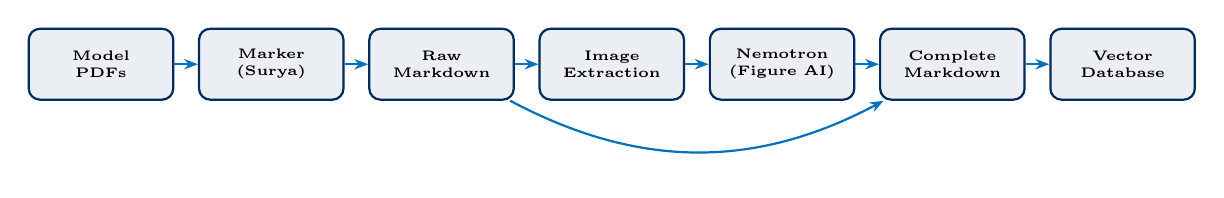
\begin{tikzpicture}[
  node distance=0.35cm and 0.3cm,
  box/.style={
    rectangle, rounded corners=4pt, draw=MSBlue, fill=MSBlue!8,
    minimum height=0.9cm, minimum width=1.75cm,
    text width=1.6cm, align=center, font=\tiny\bfseries,
    line width=0.8pt
  },
  arrow/.style={-{Stealth[length=5pt]}, thick, color=MSLightBlue},
  label/.style={font=\tiny\color{MSGrey}, align=center},
]
\node[box] (pdf) {Model\\PDFs};
\node[box, right=of pdf] (marker) {Marker\\(Surya)};
\node[box, right=of marker] (md) {Raw\\Markdown};
\node[box, right=of md] (img) {Image\\Extraction};
\node[box, right=of img] (nemotron) {Nemotron\\(Figure AI)};
\node[box, right=of nemotron] (complete) {Complete\\Markdown};
\node[box, right=of complete] (vdb) {Vector\\Database};

\draw[arrow] (pdf) -- (marker);
\draw[arrow] (marker) -- (md);
\draw[arrow] (md) -- (img);
\draw[arrow] (img) -- (nemotron);
\draw[arrow] (nemotron) -- (complete);
\draw[arrow] (md) to[bend right=28] (complete);
\draw[arrow] (complete) -- (vdb);
\end{tikzpicture}

\vspace{6pt}
\begin{columns}[T]
\begin{column}{0.48\textwidth}
  \begin{block}{\small How It Works}
    \scriptsize
    \begin{itemize}
      \item \textbf{Marker:} Converts PDF to Markdown (Surya OCR handles layout/math).
      \item \textbf{Multimodal LLM:} (e.g. Nemotron) reads charts/plots \& embeds descriptions.
      \item \textbf{Vector DB:} Stores equation-aware chunks (never split mid-formula).
    \end{itemize}
  \end{block}
\end{column}
\begin{column}{0.48\textwidth}
  \begin{block}{\small The End-State Vision}
    \scriptsize
    \begin{itemize}
      \item \textbf{Conversational Querying:} Expert answers with equation references.
      \item \textbf{Multi-Doc Comparison:} Cross-reference model specs vs. validation reports.
      \item \textbf{Accelerated Workflows:} Clean context for testing \& learning.
      \item \textbf{Code + Paper Reasoning:} Unified queries for code \& docs.
    \end{itemize}
  \end{block}
\end{column}
\end{columns}
\end{frame}

% ─── SLIDE 7: Tool Comparison & Research ────────────────────────────────────
\begin{frame}{Research Summary: Key Technologies}
\vspace{-2pt}
\small
\renewcommand{\arraystretch}{1.25}
\begin{table}[h]
\centering
\footnotesize
\begin{tabular}{p{1.6cm} p{2.5cm} p{2.6cm} p{2.2cm} p{3.2cm}}
\toprule
\textbf{Tool} & \textbf{Role} & \textbf{Strength} & \textbf{Hardware} & \textbf{Key Detail} \\
\midrule
\textcolor{MSLightBlue}{\textbf{Marker}} \newline\scriptsize{(+ Surya)} &
  \textbf{PDF $\to$ Markdown} \newline (core pipeline) &
  \iconcheck\ Best-in-class: 95.7 score &
  GPU or CPU &
  25 pages/sec on GPU; Surya is the OCR engine. \\
\textcolor{MSLightBlue}{\textbf{Docling}} \newline\scriptsize{(IBM)} &
  \textbf{PDF $\to$ Markdown} \newline (alternative) &
  \iconcheck\ Strong table extraction; MIT license &
  CPU or GPU &
  Good fallback for table-heavy documents. \\
\midrule
\textcolor{MSLightBlue}{\textbf{Nemotron}} \newline\scriptsize{(NVIDIA)} &
  \textbf{1. Figure/Image AI}\newline\textbf{2. Quant Risk Chat} &
  \iconcheck\ \textbf{1M context window}; SOTA open-model &
  Cost-effective GPUs (A10) &
  Process entire PVRMs in one pass. Ideal for both visual reasoning \& risk analysis conversations. \\
\bottomrule
\end{tabular}
\end{table}

\vspace{2pt}
\begin{exampleblock}{Strategy}
  \small \textbf{Marker} for fast document conversion on-prem. \textbf{Nemotron} for deep reasoning and figure understanding.
\end{exampleblock}
\end{frame}

% ─── SLIDE 8: Business Value ────────────────────────────────────────────────
\begin{frame}{Why This Matters: Business Value}
\begin{columns}[T]
\begin{column}{0.48\textwidth}
  \begin{block}{Speed of Validation}
    \scriptsize
    \begin{itemize}
      \item \textbf{Current:} reading 50--400 page PVRM, manually locating equations --- \textit{days/weeks}
      \item \textbf{Proposed:} natural language query in seconds.
    \end{itemize}
    \vspace{2pt}
    \renewcommand{\arraystretch}{1.1}
    \centering
    \tiny
    \begin{tabular}{lcc}
      \toprule
      \textbf{Task} & \textbf{Current} & \textbf{Proposed} \\
      \midrule
      Locate equation & 15--30\,min & $<$1\,min \\
      Cross-ref docs & 2--4\,hrs & 5--10\,min \\
      Review documentation & 1--2\,weeks & $\sim$3--5\,days \\
      Write new tests & Weeks & Days \\
      \bottomrule
    \end{tabular}
  \end{block}
\end{column}
\begin{column}{0.48\textwidth}
  \begin{block}{Broader Impact}
    \scriptsize
    \begin{itemize}
      \item \textbf{Reduce model risk:} automated consistency checks between spec and code
      \item \textbf{Replicate \& extend tests:} brainstorm new validation tests from the math
      \item \textbf{Assist in Extending \& Merging PVRMs:} Help analysts identify shared assumptions/gaps
      \item \textbf{Onboarding:} new analysts query models immediately
      \item \textbf{Audit trail:} logged queries for compliance
    \end{itemize}
  \end{block}
\end{column}
\end{columns}
\end{frame}

% ─── SLIDE 9: Implementation Phases ─────────────────────────────────────────
\begin{frame}{Implementation Phases}
\vspace{-2pt}
\centering
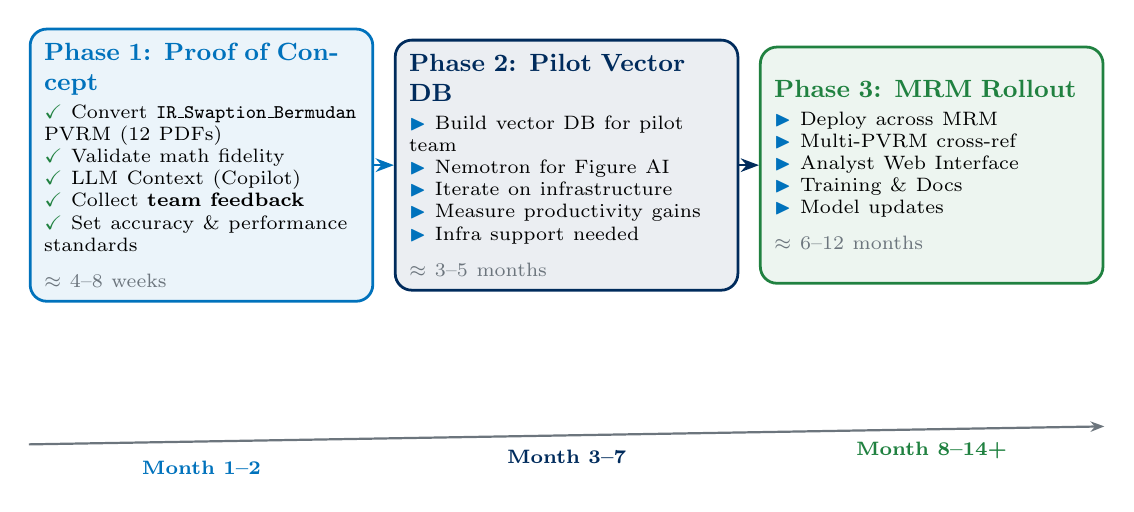
\begin{tikzpicture}

\node[phase=MSLightBlue] (p1) at (0,0) {
  \textbf{\textcolor{MSLightBlue}{Phase 1: Proof of Concept}}\\[2pt]
  \scriptsize
  \iconcheck\ Convert \texttt{IR\_Swaption\_Bermudan} PVRM (12 PDFs)\\
  \iconcheck\ Validate math fidelity\\
  \iconcheck\ LLM Context (Copilot)\\
  \iconcheck\ Collect \textbf{team feedback}\\
  \iconcheck\ Set accuracy \& performance standards\\[2pt]
  \textcolor{MSGrey}{$\approx$ 4--8 weeks}
};
\node[phase=MSBlue, right=0.25cm of p1] (p2) {
  \textbf{\textcolor{MSBlue}{Phase 2: Pilot Vector DB}}\\[2pt]
  \scriptsize
  \iconbullet\ Build vector DB for pilot team\\
  \iconbullet\ Nemotron for Figure AI\\
  \iconbullet\ Iterate on infrastructure\\
  \iconbullet\ Measure productivity gains\\
  \iconbullet\ Infra support needed\\[2pt]
  \textcolor{MSGrey}{$\approx$ 3--5 months}
};
\node[phase=AccentGreen!70!black, right=0.25cm of p2] (p3) {
  \textbf{\textcolor{AccentGreen!70!black}{Phase 3: MRM Rollout}}\\[2pt]
  \scriptsize
  \iconbullet\ Deploy across MRM\\
  \iconbullet\ Multi-PVRM cross-ref\\
  \iconbullet\ Analyst Web Interface\\
  \iconbullet\ Training \& Docs\\
  \iconbullet\ Model updates\\[2pt]
  \textcolor{MSGrey}{$\approx$ 6--12 months}
};

% Timeline
\draw[timeline] ([yshift=-1.8cm]p1.south west) -- ([yshift=-1.8cm]p3.south east);
\node[font=\scriptsize\bfseries, color=MSLightBlue] at ([yshift=-2.1cm]p1.south) {Month 1--2};
\node[font=\scriptsize\bfseries, color=MSBlue] at ([yshift=-2.1cm]p2.south) {Month 3--7};
\node[font=\scriptsize\bfseries, color=AccentGreen!70!black] at ([yshift=-2.1cm]p3.south) {Month 8--14+};

\draw[-{Stealth}, thick, MSLightBlue] (p1) -- (p2);
\draw[-{Stealth}, thick, MSBlue] (p2) -- (p3);
\end{tikzpicture}
\end{frame}

% ─── SLIDE 10: Technical Architecture ───────────────────────────────────────
\begin{frame}{Technical Architecture}
\footnotesize
\begin{columns}[T]
\begin{column}{0.48\textwidth}
  \begin{block}{1. Ingestion Pipeline}
    \begin{itemize}
      \item \textbf{PDF Ingestion:} Process via \textbf{Marker (Surya)}
      \item \textbf{Raw Markdown:} High-fidelity math extraction
      \item \textbf{Multimodal Enhancement:}
      \begin{itemize}
        \item Text \& math preserved directly
        \item Images processed by \textbf{Nemotron}
      \end{itemize}
      \item \textbf{Result:} Complete Markdown (Text + Images)
    \end{itemize}
  \end{block}

  \begin{block}{2. Dual-Store Storage}
    \begin{itemize}
      \item \textbf{Vector DB:} Equation-aware chunks for ranking
      \item \textbf{Doc Store:} Faithful Markdown for LLM context
    \end{itemize}
  \end{block}
\end{column}

\begin{column}{0.48\textwidth}
  \begin{block}{3. Query \& Retrieval Flow}
    \begin{itemize}
      \item \textbf{Retriever:} Fetches ranked chunks + full context
      \item \textbf{LLM Engine:} Nemotron generates answers
      \item \textbf{Analyst Interface:} Secure user access
    \end{itemize}
  \end{block}

  \begin{alertblock}{Security \& Compliance}
    \begin{itemize}
      \item \textbf{100\% On-Premise:} No external API calls
      \item \textbf{Open Source Stack:} Fully auditable code
      \item \textbf{Access Control:} Respects team permissions
      \item \textbf{Audit Trails:} All queries are logged
    \end{itemize}
  \end{alertblock}
\end{column}
\end{columns}
\end{frame}

% ─── SLIDE 11: Next Steps & Requirements ────────────────────────────────────
\begin{frame}{Next Steps \& Requirements}
\begin{columns}[T]
\begin{column}{0.48\textwidth}
  \begin{block}{Phase 1 Actions}
    \small
    \begin{enumerate}
      \item \textbf{Approval} to build local prototype
      \item Convert \textbf{PVRM IR\_Swaption\_Bermudan} (12~PDFs)
      \item Validate fidelity against original documents
      \item Define math fidelity score \& criteria
      \item Pilot AI assistants \& collect feedback
    \end{enumerate}
  \end{block}
\end{column}
\begin{column}{0.48\textwidth}
  \begin{block}{Resource Requirements}
    \renewcommand{\arraystretch}{1.1}
    \footnotesize
    \begin{tabular}{ll}
      \toprule
      \textbf{Resource} & \textbf{Specification} \\
      \midrule
      GPU & A10 or A100 (recommended) \\
      CPU Fallback & Possible (slower) \\
      Storage & $\sim$50\,GB \\
      Time & 4--8 weeks (Phase 1) \\
      Team & 1 engineer \\
      \bottomrule
    \end{tabular}
  \end{block}
\end{column}
\end{columns}

\vspace{10pt}
\begin{center}
\begin{minipage}{0.85\textwidth}
  \begin{exampleblock}{\centering The Ask}
    \centering\small Approval to allocate compute access and begin Phase~1 prototype on the Bermudan swaption PVRM.
  \end{exampleblock}
\end{minipage}
\end{center}
\end{frame}

% ─── SLIDE 12: Closing ──────────────────────────────────────────────────────
{
\setbeamercolor{background canvas}{bg=MSBlue}
\setbeamertemplate{footline}{}
\begin{frame}[c]
\centering
\color{MSWhite}
\Huge\bfseries Thank You\\[12pt]
\Large Questions?\\[24pt]
\normalsize
\texttt{alexander.tsoskounoglou@morganstanley.com}\\[6pt]
MRM IRD --- Budapest\\[20pt]
\small\textit{``The quality of AI output is bounded by the quality of its input.''}
\end{frame}
}

% =============================================================================
% APPENDIX — preserve frame numbering
% =============================================================================
\newcounter{savedframenumber}
\setcounter{savedframenumber}{\value{framenumber}}
\appendix
\setcounter{framenumber}{\value{savedframenumber}}

% ─── APPENDIX A: Under the Hood ─────────────────────────────────────────────
\begin{frame}{Appendix: Under the Hood}
\vspace{-2pt}
\small
\textbf{Equation:} Longstaff-Schwartz Continuation Value (Eq.~4.1)

\vspace{4pt}
\textbf{1. Original PDF}
\vspace{-2pt}
\begin{equation*}
  C(\omega; t_k) = \mathbb{E}_{\mathbb{Q}}\!\left[\sum_{j=k+1}^{K} \exp\!\left(-\int_{t_k}^{t_j} r(\omega, s)\, ds\right) I(\omega, t_j; t_k, T) \;\middle|\; \mathcal{F}_{t_k}\right]
\end{equation*}

\vspace{2pt}
\textbf{2. Standard Text Extraction} (\texttt{pymupdf4llm})
\vspace{2pt}
\fcolorbox{AccentRed}{AccentRed!5}{\parbox{0.93\textwidth}{%
\footnotesize\ttfamily\raggedright
\textcolor{AccentRed}{C(w; tk) = EQ[???? j=k+1 N exp(-- ?? rj) I(w, tj; tk, T)] ???Ftk}
}}

\vspace{4pt}
\textbf{3. High-Fidelity Pipeline} (\texttt{Marker/Surya})
\vspace{2pt}
\fcolorbox{AccentGreen}{AccentGreen!5}{\parbox{0.93\textwidth}{%
\footnotesize\ttfamily\raggedright
\textcolor{black}{%
\$\$C(w; t\_k) = \textbackslash mathbb\{E\}\_\{\textbackslash mathbb\{Q\}\} \textbackslash Big[ \textbackslash sum\_\{j=k+1\}\^{}\{K\}
exp \textbackslash Big( - \textbackslash int\_\{t\_k\}\^{}\{t\_j\} r(w, s) \textbackslash\ ds \textbackslash Big) I(w, t\_j; t\_k, T) \ldots\$\$}%
}}
\end{frame}

% ─── APPENDIX B: Marker Benchmarks ──────────────────────────────────────────
\begin{frame}{Appendix: Marker Benchmark Performance}
\small
\renewcommand{\arraystretch}{1.2}
\begin{table}[h]
\centering
\footnotesize
\begin{tabular}{lccc}
\toprule
\textbf{Method} & \textbf{Time (sec)} & \textbf{Heuristic Score} & \textbf{LLM Score} \\
\midrule
\textbf{Marker} & \textbf{2.84} & \textbf{95.67} & \textbf{4.24} \\
Docling & 3.70 & 86.71 & 3.70 \\
Mathpix & 6.36 & 86.43 & 4.16 \\
LlamaParse & 23.35 & 84.24 & 3.98 \\
\bottomrule
\end{tabular}
\caption{Benchmark data from Marker GitHub repository.}
\end{table}

\vspace{4pt}
\begin{columns}[T]
\begin{column}{0.48\textwidth}
  \begin{block}{\small Throughput}
    \scriptsize
    \begin{itemize}
      \item Single-page serial: 2.84\,s
      \item Batch mode on H100: \textbf{25 pages/sec}
      \item Can run on \textbf{A10, V100, MPS, or CPU}
    \end{itemize}
  \end{block}
\end{column}
\begin{column}{0.48\textwidth}
  \begin{block}{\small By Document Type (Heuristic)}
    \scriptsize
    \begin{tabular}{lc}
      Scientific paper & 96.67 \\
      Financial document & 95.37 \\
      Legal document & 96.69 \\
    \end{tabular}
    \vspace{2pt}
    
    \textbf{Financial documents} score 95.4/100.
  \end{block}
\end{column}
\end{columns}
\end{frame}

% ─── APPENDIX C: Cost & Productivity Analysis ───────────────────────────────
\begin{frame}{Appendix: Cost \& Productivity Estimation}
\vspace{-8pt}
\scriptsize

\begin{columns}[T]
\begin{column}{0.48\textwidth}
  \begin{block}{\scriptsize Cost per Query}
    \renewcommand{\arraystretch}{1.05}
    \tiny
    \textbf{Platform:} Microsoft Azure (MS strategic partner)\\[2pt]
    \begin{tabular}{p{2.0cm} r r}
      \toprule
      \textbf{Model} & \textbf{In/1M} & \textbf{Out/1M} \\
      \midrule
      Nemotron-3-Nano \newline \textcolor{MSGrey}{(open-source)} & \$0.05 & \$0.20 \\
      Gemini 3 Pro \newline \textcolor{MSGrey}{(closed, SOTA)} & \$2.00 & \$12.00 \\
      \bottomrule
    \end{tabular}

    \vspace{2pt}
    \textbf{Typical query:} $\sim$4k input + $\sim$1.5k output tokens\\[1pt]
    \iconbullet\ Nemotron-3-Nano: \textcolor{AccentGreen!70!black}{\textbf{\$0.0005}}/query\\
    \iconbullet\ Gemini 3 Pro: \textcolor{MSLightBlue}{\textbf{\$0.026}}/query
  \end{block}
\end{column}

\begin{column}{0.48\textwidth}
  \begin{block}{\scriptsize Monthly Cost Projection (per analyst)}
    \renewcommand{\arraystretch}{1.05}
    \tiny
    \textbf{Est.\ queries:} 25--40/day $\times$ 22 days/month\\[2pt]
    \begin{tabular}{l r r r}
      \toprule
      \textbf{Scenario} & \textbf{Q/day} & \textbf{Nano} & \textbf{Gemini 3} \\
      \midrule
      Conservative & 25 & \$0.28 & \$14.30 \\
      Normal & 35 & \$0.39 & \$20.02 \\
      Heavy use & 50 & \$0.55 & \$28.60 \\
      \bottomrule
    \end{tabular}

    \vspace{2pt}
    \textbf{Team of 10 (Gemini 3):} \textcolor{AccentGreen!70!black}{\textbf{\$143--286/month}}
  \end{block}
\end{column}
\end{columns}

\vspace{2pt}
\begin{block}{\scriptsize Estimated Efficiency Gains per PVRM Revalidation}
  \renewcommand{\arraystretch}{1.05}
  \tiny
  \begin{tabular}{p{3.0cm} c c c c}
    \toprule
    \textbf{Task} & \textbf{Current} & \textbf{Conservative} & \textbf{Normal} & \textbf{Optimistic} \\
    \midrule
    Read \& digest PVRM docs & $\sim$16--24\,hrs & $-$10\% (\textbf{14--22\,h}) & $-$20\% (\textbf{13--19\,h}) & $-$30\% (\textbf{11--17\,h}) \\
    Locate equations/sections & $\sim$2--4\,hrs & $-$15\% (\textbf{1.7--3.4\,h}) & $-$25\% (\textbf{1.5--3\,h}) & $-$40\% (\textbf{1.2--2.4\,h}) \\
    Cross-reference documents & $\sim$4--8\,hrs & $-$15\% (\textbf{3.4--6.8\,h}) & $-$30\% (\textbf{2.8--5.6\,h}) & $-$45\% (\textbf{2.2--4.4\,h}) \\
    Interpret figures \& tables & $\sim$2--4\,hrs & $-$10\% (\textbf{1.8--3.6\,h}) & $-$20\% (\textbf{1.6--3.2\,h}) & $-$35\% (\textbf{1.3--2.6\,h}) \\
    Draft validation tests & $\sim$40--80\,hrs & $-$10\% (\textbf{36--72\,h}) & $-$20\% (\textbf{32--64\,h}) & $-$30\% (\textbf{28--56\,h}) \\
    \midrule
    \textbf{Total per PVRM} & \textbf{$\sim$64--120\,hrs} & $-$\textbf{12\%} & $-$\textbf{22\%} & $-$\textbf{35\%} \\
    \bottomrule
  \end{tabular}
\end{block}

\vspace{1pt}
\centering
\tiny\textcolor{MSGrey}{Pricing: Azure AI Foundry (Feb 2026). Assumes RAG-based retrieval. Speed-ups assume high-fidelity extraction pipeline is deployed.}
\end{frame}

\end{document}
